首先分治的做法是众所周知的。

有期望 $O(n)$ 的随机增量法:首先将所有点随机打乱,然后每次增加一个点,更新答案。

假设当前最近点对距离为 $s$,则把平面划分成 $s \times s$ 的方格,用哈希表存储每个方格有哪些点。

加入一个新点时,只需要枚举自身和周围共计 $9$ 个方格中的点,显然枚举到的点最多 $16$ 个。如果加入之后答案变小了,就 $O(n)$ 暴力重构。

前 $i$ 个点中 $i$ 是最近点对中的点的概率至多为 $\frac 2 i$,所以每个点的期望贡献都是 $O(1)$,总的复杂度就是期望$O(n)$。

如果对每个点都要求出距离最近的点的话,也有随机化的 $O(n)$ 做法:

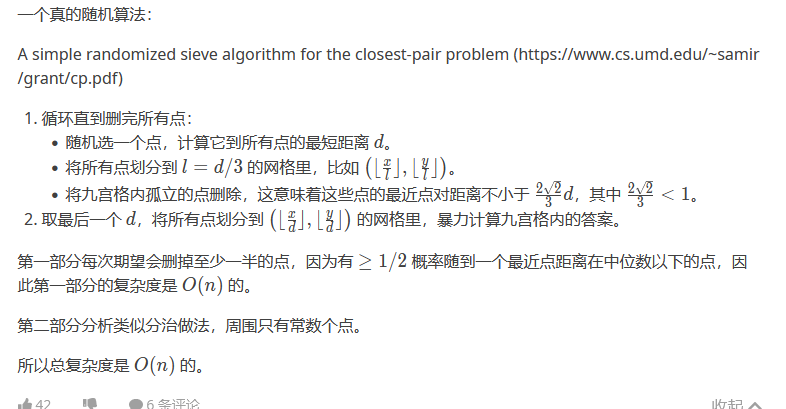
\includegraphics[width=0.8\linewidth]{../src/geometry/最近点对.png}
